\documentclass[paper=a4, parskip=half]{scrreprt}

\usepackage{etex}
\usepackage[utf8]{inputenc}
\usepackage[T1]{fontenc}

\usepackage{lmodern}
\usepackage[ngerman]{babel}

\usepackage{bibgerm} 
\usepackage{cite}
\usepackage{url}

\usepackage{graphics}

\usepackage[hypertexnames=false, linktocpage]{hyperref}

\usepackage{titling}
\usepackage{graphicx}
\graphicspath{ {./Bilder/} }
\usepackage{wrapfig}
\usepackage{float}
\usepackage{adjustbox}
\usepackage{setspace}
\usepackage[acronym]{glossaries}
\usepackage{datetime}

\usepackage{subfiles} % Best loaded last in the preamble

\subfile{Meta/glossary}

\setcounter{tocdepth}{1}

\begin{document}
%TC:ignore
\title{Aktivitaetsdiagramm} % Meta

\subfile{Meta/coversheet}
\subfile{Meta/guides}


%TC:endignore
\chapter{Aktivitätsdiagramm}
% Grafik
\begin{adjustbox}{center,caption=
		{UML-Aktivitätsdiagramm für Genderly}
		,label={UML-Aktivitätsdiagramm für Genderly} ,nofloat=figure,vspace=\bigskipamount}
	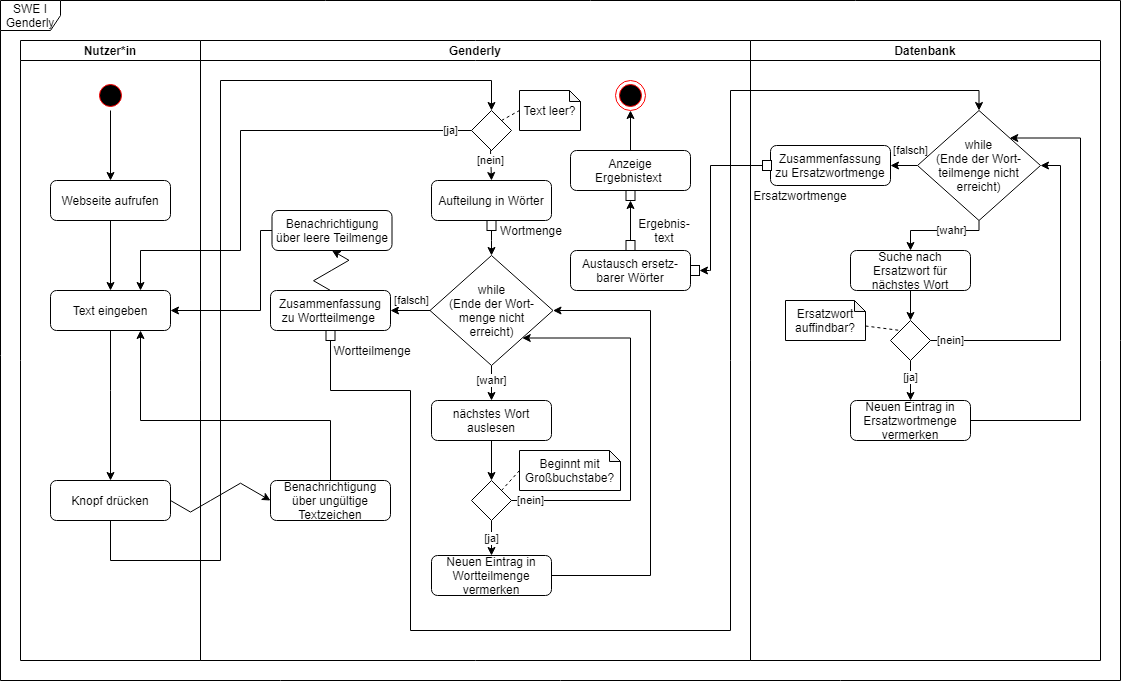
\includegraphics[width=\textwidth]{Bilder/Diagramme/Aktivitaetsdiagramm.png}
\end{adjustbox}
\vspace{0.25cm}
\chapter{Beschreibung}
Der vorliegend mit dem Aktivitätsdiagramm beschriebene Prozess aus Textaufnahme, Verarbeitung und Ausgabe bildet die Kernkompetenz der Anwendung \textsc{Genderly}. Bei \textsc{Genderly} handelt es sich um eine Webanwendung. Der Prozess kann entsprechend während der Laufzeit beliebig oft wiederholt werden, da der Web-Server nach Prozessende weiterläuft.\\
Eine Interaktion beginnt mit dem Öffnen der Weboberfläche durch eine*n Nutzer*in, sowie die nutzer*innenseitige Texteingabe eines syntaktisch korrekten, deutschen Texts. Sobald ein Knopf gedrückt wird, erfährt der Text eine Prüfung auf ungültige Zeichen, z.B. Steuerzeichen des ASCII-Zeichensatzes. Sollte Derartiges im Text gefunden werden, oder gar ein leerer Text vorliegen, wird der Nutzer bzw. die Nutzerin um wiederholte Eingabe gebeten.\\
Ein für gültig befundener, eingelesener Text wird in eine Menge aus Wörtern zerlegt. Von dieser Menge wird eine Teilmenge aus allen Wörtern gebildet, die mit einem Großbuchstaben beginnen. Diese Menge umfasst allgemein in deutschen Texten zwingend die Wortteilmenge der Substantive, enthält u.U. aber auch z.B. Artikel oder Wörter an Satzanfängen. Diese Teilmenge darf nicht leer sein, wenn es sich um geforderte, syntaktisch korrekte Texte handelt. Sollte sie leer sein, wird der Nutzer bzw. die Nutzerin erneut um Eingabe gebeten.\\
Die Wortteilmenge wird an eine Datenbank weitergeleitet. Sie versucht nun pro Wort eine Menge vermerkter Ersatzwörter zu finden. Diese Menge wird dem Ausgangswort zugewiesen. Wiederum diese Zuordnung von Wort zu Ersatzwortmenge wird einer globalen Ersatzwortmengen-Struktur hinzugefügt. Mit den Aufschlüssen aus dieser Struktur werden die ersetzbaren Wörter nun ersetzt. Der aus alten Satzteilen und Ersatzwörtern zusammengesetzte, neue Text wird abschließend angezeigt.
\\
\\
\begin{tiny}
Wortanzahl: 241
\end{tiny}

%TC:ignore

%Glossar
%\printglossary
%\pagebreak

%\nocite{*}
%\bibliography{Literatur}
%\bibliographystyle{alphadin}


%\subfile{Anhang/main}
%TC:endignore

\end{document}